
\section{Généralités}

Afin de garantir l’homogénéité et la qualité des livrables, il est nécessaire de définir un cycle de vie des documents. Ainsi, chaque document devant être produit au cours du projet devra respecter les différentes étapes dudit cycle de vie. Lorsqu’un nouveau document entre en production au sein du projet, celui-ci sera soumis à deux phases principales. La première correspond à la procédure interne de vérification, réalisée par l’équipe, de façon collaborative, et visant à vérifier le contenu du document. La seconde phase correspond à la procédure de recette client, réalisée par le responsable qualité et par le chef de projet, permettant ainsi de valider le document en vérifiant notamment la mise en forme. L’enchaînement global des étapes au sein des phases est représenté dans le schéma ci-dessous, tandis que le détail de chaque phase est explicité à travers les sous-paragraphes ci-après.

\begin{figure}[H]
    \centering
    \label{fig-valid-recette}
    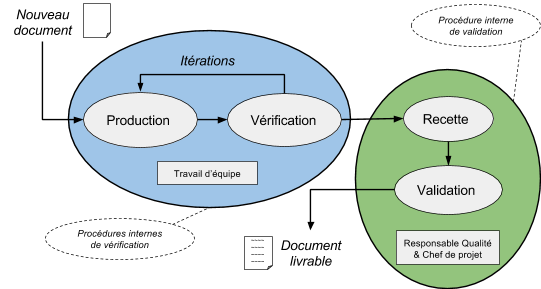
\includegraphics[scale=0.5]{figures/validation_recette.png}
    \caption{Procédures complètes de validation et de recette}
\end{figure}

\section{Procédure interne de vérification}
    
Lorsqu’un nouveau document doit être établi, celui-ci entre directement dans la phase de procédure interne de vérification. Le document est alors créé grâce à l’outil Google Docs évoqué précédemment, en mode partagé afin que tous les collaborateurs disposent d’un accès à celui-ci. Afin de disposer d’un suivi avancé sur le document, un cartouche est directement apposé sur la première page de ce nouveau document. Le format du cartouche est alors le suivant : \\

\begin{figure}[H]
\centering
\label{fig-cartouche}
\scalebox{0.8}{
\begin{tabular}{|m{0.3\textwidth}|m{0.3\textwidth}|m{0.3\textwidth}|}
  \hline
  \textbf{Auteurs du document} & \textbf{Relecteur} & \textbf{Responsable qualité} \\
  \hline
   & & \rule[0cm]{0cm}{3cm} \\
  \hline
\end{tabular}
}
\caption{Modèle de cartouche présent sur les documents livrés}
\end{figure}

Après ajout de ce cartouche, le document passe alors dans l’étape de \og{}production-rédaction\fg{}. Chaque collaborateur peut alors modifier et améliorer le document, en fonction de ses compétences et expertises. Lorsqu’un nouveau collaborateur contribue à l’amélioration du document, celui-ci a l’obligation d’ajouter son nom dans le cartouche, à l’emplacement intitulé \og{}Auteurs du document\fg{}. \\
 
Des vérifications sont également effectuées à intervalles réguliers sur le document par les différents acteurs qui, s'ils sont satisfaits, valident leur étape de production en signant le cartouche, à l’emplacement prévu, situé sous l’intitulé \og{}Auteurs du document\fg{}. Ils en informent alors le relecteur assigné du document. Ce dernier doit impérativement être extérieur à la réalisation du document, afin de garantir une impartialité d’opinion sur le contenu de celui-ci. \\
 
Ensuite, l’étape de vérification est effectuée dans un premier temps par le relecteur assigné, puis par le responsable qualité. Le relecteur passe le document en mode “suggestion” sur Google Document, permettant ainsi de mettre en valeur les passages modifiés. Si le contenu est correct, le document passe en phase de validation A contrario, en présence d’erreurs ou d’incohérences, le document retourne à l’étape de production. Afin d'effectuer le suivi du document, une nouvelle ligne est ajoutée au cartouche. \\
 
L’enchaînement des étapes de cette phase du cycle de vie des documents est représenté à travers le schéma ci-dessous. \\

\begin{figure}[H]
    \centering
    \label{fig-valid}
    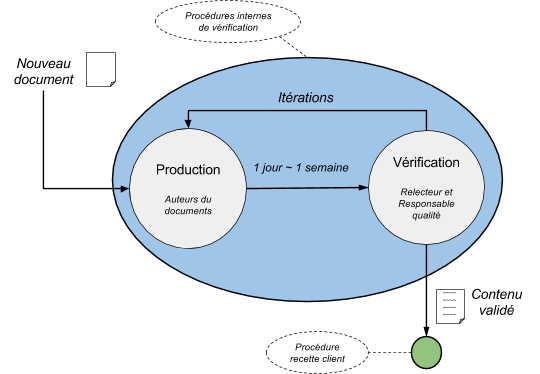
\includegraphics[scale=0.5]{figures/validation_part.png}
    \caption{Procédure de validation}
\end{figure}

\section{Procédures internes de validation}
    
Lorsqu’un document termine sa phase de procédure interne de vérification, celui-ci débute la phase de procédure de recette client. Cette phase consiste à transformer le document collaboratif, sans mise en forme initiale, en un document répondant aux critères de qualité et respectant un format défini, à l’aide du format LaTeX. Cette étape de transformation, ou recette, est réalisée par le responsable qualité, qui veille à respecter les standards définis au préalable, afin de garantir l’uniformité des livrables. Après réalisation de cette étape, le responsable qualité appose sa signature sur le cartouche, à l’emplacement situé sous l’intitulé « Responsable qualité ». \\
 
Le document débute alors la dernière étape de son cycle de vie, qui correspond à la validation. Cette étape permet de garantir une dernière fois la bonne mise en forme du document, tout en déclarant le document terminé après avoir réalisé une dernière relecture, empêchant ainsi toute retouche par la suite. Cette étape est réalisée conjointement par le responsable qualité et par le chef de projet. Le document devient alors un document livrable, au format PDF, pouvant être archivé et livré au client. \\
 
Le déroulement de cette phase de recette client est résumé à travers le schéma ci-dessous.

\begin{figure}[H]
    \centering
    \label{fig-recette}
    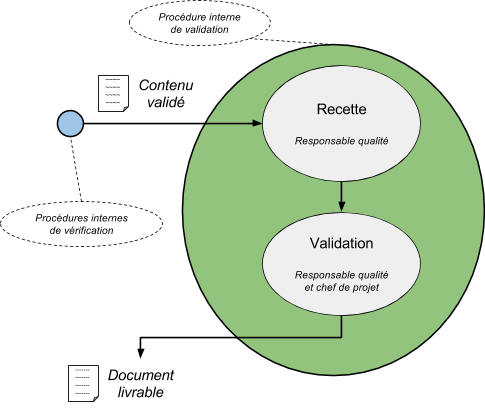
\includegraphics[scale=0.5]{figures/recette_part.png}
    \caption{Procédure de recette}
\end{figure}

\section{Procédure de recette externe}

Lorsqu’un document est considéré comme étant livrable, ce dernier doit être soumis au client. Afin d’attester ladite livraison à une date donnée, prouvant ainsi le respect des délais, un procès-verbal de livraison est édité. Ainsi, le chef de projet modifie le document type disponible en Annexe A, adaptant ce dernier au livrable devant être fourni au client. Les informations importantes à mentionner dans ces procès-verbaux de livraison sont les suivantes : \\

\begin{itemize}
    \item[\textbullet] Référence et intitulé du livrable
    \item[\textbullet] Récepteur du livrable : nom et signature
    \item[\textbullet] Émetteur du livrable : nom et signature
    \item[\textbullet] Date de la livraison \\
\end{itemize}

Ces procès-verbaux de livraison sont produits en double exemplaire, permettant ainsi à l’émetteur et au récepteur du livrable de posséder une attestation de remise. Les deux partis s’engagent ainsi, par leur signature, à clôturer le cycle de vie du document livré, ce dernier ne pouvant être retouché par la suite.
